
\subsection{What Happened}

\subsubsection{Primary Venue Execution — Explained}

This is the first and preferred route your algorithm uses to send trades. Think of it as the 
“main road” in a trading network:

\begin{itemize}
  \item \textbf{High-liquidity:} These venues (like NYSE, NASDAQ, ARCA) usually have a lot of buyers and 
  sellers, so trades can happen quickly with minimal price movement.
  \item \textbf{Low-latency:} These exchanges are fast — orders are matched in milliseconds or less, and 
  feedback is nearly instantaneous.
\end{itemize}

\textbf{What Went Wrong — Step by Step}

\paragraph{Top bids were pulled:} This means that the best offers to buy (the top of the bid stack on 
the depth ladder) suddenly disappeared — market participants (likely market makers) withdrew their interest. 
This can happen during stress, uncertainty, or if they detect hidden risk.

This means that the highest prices offered to buy an asset — the most aggressive buyers in the order book — 
suddenly disappeared. These are typically market makers, who provide liquidity by constantly posting bids and 
offers. Their presence keeps spreads tight and execution costs low.

But under stress — say, during a geopolitical headline, unexpected data release, or signs of structural risk — 
these market makers can withdraw in seconds. When they do, the visible depth evaporates. The book still “looks 
alive,” but the best-priced liquidity is gone.

As an example, imagine you're at an auction where dozens of people are loudly bidding on a painting.

Suddenly, someone whispers that the painting might be a forgery.

In seconds, all the loudest bidders — the ones who were offering the most — step back.

The auctioneer is still on stage. The lights are still on. But the high bids are gone.

It looks like an auction. It sounds like an auction.
But you’re about to sell into silence.

In trading terms, the top of the depth ladder just vanished — and unless your system recognizes that the noise is gone, 
you’ll still route orders as if someone’s there to catch them.

That’s what happened here.


\begin{figure}[H]
  \centering
  \resizebox{0.9\textwidth}{!}{%
    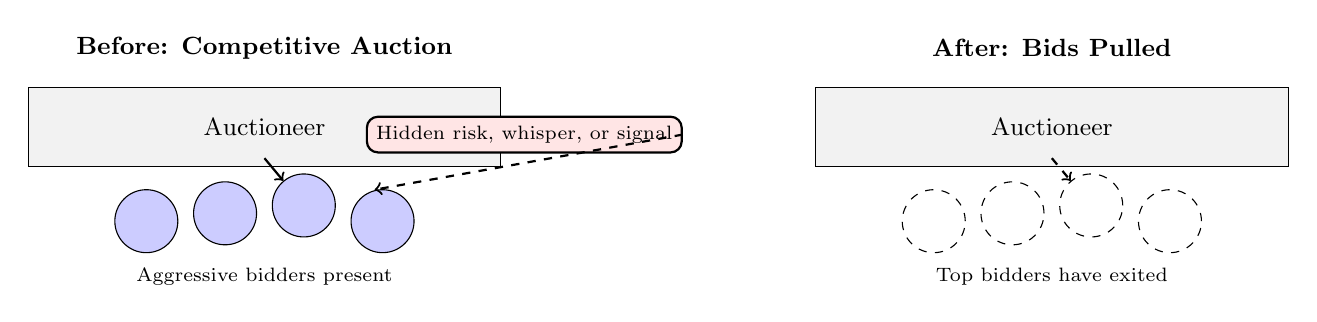
\begin{tikzpicture}[
      font=\small,
      person/.style={circle, draw, minimum size=0.8cm, fill=blue!20},
      personfaded/.style={circle, draw, minimum size=0.8cm, fill=white, dashed},
      stage/.style={rectangle, draw, minimum width=6cm, minimum height=1.0cm, fill=gray!10},
      label/.style={font=\scriptsize\itshape},
      whisper/.style={rectangle, draw, thick, rounded corners, fill=red!10, font=\scriptsize},
      arrow/.style={->, thick}
    ]

    % Titles
    \node at (-5, 5.2) {\textbf{Before: Competitive Auction}};
    \node at (5, 5.2) {\textbf{After: Bids Pulled}};

    % Auction stages
    \node[stage] (stageL) at (-5, 4.2) {Auctioneer};
    \node[stage] (stageR) at (5, 4.2) {Auctioneer};

    % Bidders - Before
    \node[person] (p1) at (-6.5,3.0) {};
    \node[person] (p2) at (-5.5,3.1) {};
    \node[person] (p3) at (-4.5,3.2) {};
    \node[person] (p4) at (-3.5,3.0) {};
    \node at (-5,2.3) {\scriptsize Aggressive bidders present};

    % Bidders - After
    \node[personfaded] (f1) at (3.5,3.0) {};
    \node[personfaded] (f2) at (4.5,3.1) {};
    \node[personfaded] (f3) at (5.5,3.2) {};
    \node[personfaded] (f4) at (6.5,3.0) {};
    \node at (5,2.3) {\scriptsize Top bidders have exited};

    % Arrows from auctioneer to bidders
    \draw[arrow] (-5,3.8) -- (p3);
    \draw[arrow, dashed] (5,3.8) -- (f3);

    % Whisper box
    \node[whisper] (rumor) at (-1.7,4.1) {Hidden risk, whisper, or signal};

    % Whisper arrow
    \draw[->, thick, dashed] (rumor.east) -- (-3.6,3.4);

    \end{tikzpicture}%
  }
  \caption{Auction Metaphor: Before the top bids were pulled, the system saw an active market. But when aggressive bidders withdrew, 
  the structure remained — even as the interest vanished.}
\end{figure}




\paragraph{Depth vanished:} Below those top five bids, there was no real liquidity. The order book looked 
healthy on the surface, but there was no meaningful volume to execute against.

The term “depth” refers to the amount of buy and sell interest in an order book beyond just the top bid or ask. A deep book means 
there's real volume to back up pricing — not just surface-level quotes.

In this case, below the top five bids, there was nothing of substance. The order book still appeared functional — it had prices, 
rows, and levels — but the actual quantity available to trade at those prices had thinned out or disappeared entirely.

Imagine walking into a grocery store that looks fully stocked from the entrance. The shelves are neatly labeled: "Pasta – \$2.99", 
"Soup – \$1.49", "Olive Oil – \$8.99".

But when you walk down the aisle and reach for the items, the shelves are empty.

Everything looks normal from a distance. The signs are there. The aisles are lit. The music is playing.
But the food is gone.

That’s what “depth vanished” means in trading.

The order book still had quotes — but they weren’t backed by real liquidity. It gave the illusion of market health. So when the 
algorithm tried to execute, it fell through a hollow layer — like stepping onto a stair that isn’t actually there.


\begin{figure}[H]
  \centering

  % === First row ===
  \begin{subfigure}[t]{0.45\textwidth}
    \centering
    \begin{tikzpicture}
      \comicpanel{0}{0}
        {Trader}
        {Algo}
        {\small Bid stack shows 5 levels. Spread is 1.2 bps. Latency normal.}
        {(-0.6,-0.6)}
    \end{tikzpicture}
    \caption*{It looked like a fully stocked store from the entrance.}
  \end{subfigure}
  \hfill
  \begin{subfigure}[t]{0.45\textwidth}
    \centering
    \begin{tikzpicture}
      \comicpanel{0}{0}
        {Trader}
        {Algo}
        {\small Execute 80{,}000 shares via primary. Use sweep logic on trigger.}
        {(0.6,-0.6)}
    \end{tikzpicture}
    \caption*{They tried to check out with a full cart.}
  \end{subfigure}

  \vspace{1em}

  % === Second row ===
  \begin{subfigure}[t]{0.45\textwidth}
    \centering
    \begin{tikzpicture}
      \comicpanel{0}{0}
        {Algo}
        {Trader}
        {\small Fill rate 23\%. Slippage 38 bps. Remaining order re-queued.}
        {(-0.6,-0.6)}
    \end{tikzpicture}
    \caption*{The scanner beeped — but the bags were empty.}
  \end{subfigure}
  \hfill
  \begin{subfigure}[t]{0.45\textwidth}
    \centering
    \begin{tikzpicture}
      \comicpanel{0}{0}
        {Trader}
        {Algo}
        {\small Copy. Treat primary venue as behavioral void. Failover to synthetic.}
        {(0.6,-0.6)}
    \end{tikzpicture}
    \caption*{The shelves were labeled. The lights were on. But the store was a hologram.}
  \end{subfigure}

  \caption*{\textbf{Depth Vanished:} The system saw structure. It mistook labels for substance.}
\end{figure}


\paragraph{Silent failure:} Here’s the critical flaw: the system didn’t see this as a failure.

Here’s the critical flaw: the system didn’t see this as a failure.

Everything about the venue appeared normal. Orders were being accepted. Latency was low. No errors. 
No rejections. The technical indicators — the ones the system was trained to watch — all said green.

So the aggregator kept routing trades there. And the trades kept slipping. Quietly. Repeatedly.

Slippage is when a trade executes at a worse price than expected.

You place an order expecting to buy at, say, \$100 — because that’s what the top bid or ask shows 
in the book. But by the time your order actually hits the market, that price has vanished, and you 
end up buying at \$100.42.

That 42 cents?
That’s slippage.

In a deep, healthy market, slippage is minimal — just a few basis points. But when liquidity thins, 
or when the visible quotes are illusions, slippage balloons. You think you're buying at market — but 
the market is evaporating beneath your feet.

Example (Grocery Store Analogy):
Imagine walking into a pristine grocery store.

The lights are on.

The shelves are labeled.

The scanners beep.

The receipts print.

You fill your cart. You head to checkout.
You swipe your card.
The screen says: “Transaction approved.”

But here’s the catch:
None of the bags have food in them.

No one told you. No one flagged it. The barcode scanner beeped, but it wasn’t connected to anything. 
The system was technically working, but it was functionally useless.

You walk out of the store with empty bags and a receipt that says you bought “groceries.”

That’s what a silent failure looks like.

In trading terms, the order book still responded. The venue still accepted orders. But there was 
no meaningful liquidity to fill those orders.

The system didn’t crash.
It just kept doing its job — executing perfectly into nothing.

\begin{figure}[H]
  \centering
  \resizebox{0.85\textwidth}{!}{%
    \begin{tikzpicture}[
      font=\small,
      venue/.style={draw, thick, fill=gray!10, rounded corners, minimum width=4.2cm, minimum height=1.2cm, align=center},
      state/.style={draw, thick, minimum width=4.2cm, minimum height=1.2cm, rounded corners=4pt, align=center},
      arrow/.style={->, thick},
      label/.style={font=\scriptsize\itshape},
      bidbox/.style={rectangle, draw=black, fill=blue!20, minimum width=0.6cm, minimum height=0.4cm},
      fadedbox/.style={rectangle, draw=black, dashed, fill=white, minimum width=0.6cm, minimum height=0.4cm}
    ]

    % Labels
    \node at (-4, 5.4) {\textbf{Primary Venue Execution — Intended}};
    \node at (4.5, 5.4) {\textbf{What Went Wrong — Step by Step}};

    % Intended Flow
    \node[venue] (intended) at (-4, 4.4) {Primary Venue (e.g. NYSE)};
    \node[state, below=0.9cm of intended] (liquidity) {High Liquidity\\+ Low Latency};
    \draw[arrow] (intended) -- (liquidity);

    \node[label, below=0.2cm of liquidity] {“Main road” execution};

    % Failure stages
    \node[state] (topbids) at (4.5, 4.4) {
      \textbf{Top Bids Pulled}\\
      Market makers step back
    };

    \node[state, below=0.9cm of topbids] (depth) {
      \textbf{Depth Vanished}\\
      Order book hollow below
    };

    \node[state, below=0.9cm of depth] (silentfail) {
      \textbf{Silent Failure}\\
      No alert triggered
    };

    \draw[arrow] (topbids) -- (depth);
    \draw[arrow] (depth) -- (silentfail);

    % Order book diagram
    \node at (-4, 1.2) {\textbf{Order Book View}};

    % Functioning order book
    \foreach \i in {0,...,4} {
      \node[bidbox] at (-5.2 + \i*0.65, 0.3) {};
    }

    % Failed order book (ghost bids)
    \foreach \i in {0,...,1} {
      \node[fadedbox] at (3.2 + \i*0.65, 0.3) {};
    }

    \foreach \i in {2,...,4} {
      \node[draw=none, fill=none] at (3.2 + \i*0.65, 0.3) {}; % Empty space (no depth)
    }

    \node[label] at (-4, -0.3) {Normal: Tight spreads, deep book};
    \node[label] at (4.5, -0.3) {Failure: Top bids gone, depth empty};

    \end{tikzpicture}%
  }
  \caption{Primary Venue Execution: The system was designed to route through fast, liquid venues — but failed to recognize the collapse of depth and liquidity as a critical failure.}
\end{figure}


There was no technical error (the venue was still online).

Latency monitors — tools that check how quickly orders are acknowledged or rejected — were still within normal 
bounds.

So no alarms went off.

The execution engine kept sending trades into a “healthy” venue that was, in reality, hollow. The system saw 
normal timing and no rejected orders — so it assumed everything was fine.

\textbf{Why was no flag triggered?}  Most monitoring systems watch for:

\begin{itemize}
  \item Order rejections
  \item Latency spikes
  \item Venue unresponsiveness
\end{itemize}

But here, the venue was technically functioning.
The problem was \textbf{behavioral}, not technical.

The liquidity had evaporated — the goods were gone — but the infrastructure was still “on.”
Shelves still had price tags. Checkout scanners still beeped. The receipt still printed.

So to the system, nothing looked broken — even though execution quality was degrading fast.

\textbf{Analogy}
Imagine walking into a grocery store:

The lights are on.

The music is playing.

The aisles are clean.

The scanner beeps.

The shelves are labeled.

But there’s no food.
Everything that matters is gone — quietly, systemically, without a sign.

And the store doesn’t flag this as a problem.

Your basket fills with items that aren’t there.
Your receipt shows prices that no longer exist.
And the system thinks the store is fully operational — because the scanner still works and no one tripped the alarm.

That’s what behavioral failure looks like:
It’s not that the system broke. It’s that it kept functioning long after it became useless.



\begin{figure}[H]
  \centering
  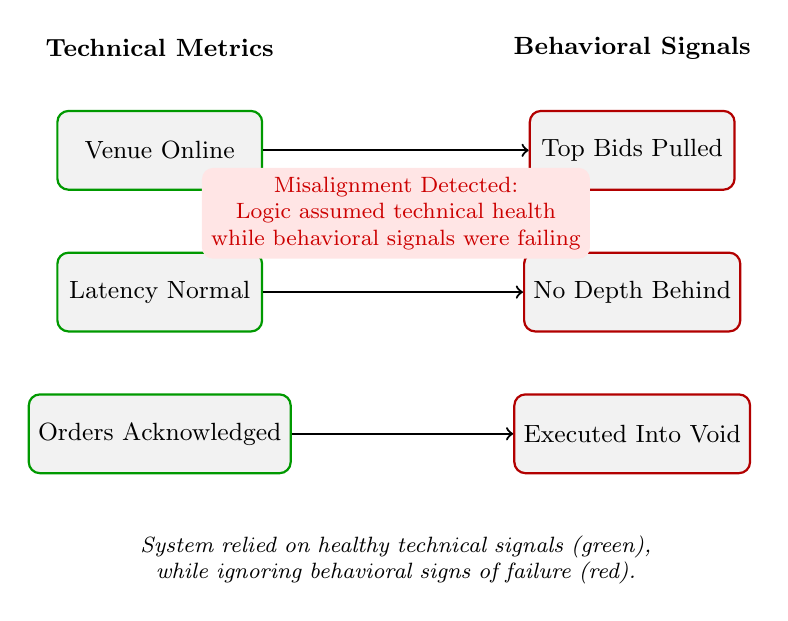
\begin{tikzpicture}[
      every node/.style={font=\small},
      component/.style={draw, rounded corners, minimum width=2.6cm, minimum height=1cm, fill=gray!10},
      healthy/.style={draw=green!60!black, thick},
      warning/.style={draw=red!70!black, thick},
      arrow/.style={->, thick}
    ]

    % Technical Metric Boxes (left column)
    \node[component, healthy] (venueUp) at (0,4) {Venue Online};
    \node[component, healthy] (latency) at (0,2.2) {Latency Normal};
    \node[component, healthy] (ack) at (0,0.4) {Orders Acknowledged};

    % Behavioral Signal Boxes (right column)
    \node[component, warning] (bidsPulled) at (6,4) {Top Bids Pulled};
    \node[component, warning] (depthGone) at (6,2.2) {No Depth Behind};
    \node[component, warning] (execVoid) at (6,0.4) {Executed Into Void};

    % Annotations
    \node at (0,5.3) {\textbf{Technical Metrics}};
    \node at (6,5.3) {\textbf{Behavioral Signals}};
    \node[align=center, font=\footnotesize, text width=9cm] at (3,-1.2) {
      \textit{System relied on healthy technical signals (green), \\ while ignoring behavioral signs of failure (red).}
    };

    % Arrows between aligned layers
    \draw[arrow] (venueUp.east) -- (bidsPulled.west);
    \draw[arrow] (latency.east) -- (depthGone.west);
    \draw[arrow] (ack.east) -- (execVoid.west);

    % Problem annotation
    \node[draw=none, fill=red!10, rounded corners, text=red!80!black, font=\footnotesize, align=center] at (3,3.2)
    {Misalignment Detected: \\ Logic assumed technical health \\ while behavioral signals were failing};

  \end{tikzpicture}
  \caption{Behavioral vs. Technical Metrics — Why Latency and Acknowledgments Can Miss Real Market Stress}
\end{figure}


\textbf{Synthetic Aggregator Layer — Misreading Structural Withdrawal}

The \textbf{Synthetic Aggregator Layer} is a smart-routing system that reconstructs best execution by stitching 
together partial fills across multiple smaller venues. Its core logic:

\begin{itemize}
  \item Break large orders into smaller tranches.
  \item Route tranches across diverse venues.
  \item Reassemble fills to approximate best price and speed.
\end{itemize}

\textbf{Break large orders into smaller tranches — Explained}

When a trading algorithm receives a large order — say, to buy 1 million shares of a stock — it doesn’t just fire 
that order into the market all at once. Doing so would cause an immediate price impact: the order would overwhelm 
available supply at the best prices, drive up the cost of the trade, and potentially signal intent to the rest 
of the market.

Instead, the system \textbf{slices} that large order into smaller, more manageable pieces — called tranches.

A tranche might be 5,000 shares, 1,000 shares, or even 100 — the size depends on market conditions, liquidity, 
urgency, and risk constraints.

What determines tranche size?

\begin{itemize}
  \item \textbf{Market Conditions:} Is the stock stable or volatile? In calm markets, larger tranches are safer. 
  In choppy markets, smaller ones help avoid getting caught in sudden swings.

  \item \textbf{Liquidity:} How many buyers and sellers are available? If there’s lots of activity and deep 
  order books, the algorithm can afford to send bigger chunks. If there’s barely anyone on the other side, 
  it has to go slow and small.

  \item \textbf{Urgency:} Does the order need to be filled fast, or can it wait? Urgent trades may sacrifice 
  price to get speed, while slower trades use smaller tranches to tiptoe through the market and minimize footprint.

  \item \textbf{Risk Constraints:} Are there internal limits on how much exposure the firm wants at any given 
  moment? Algorithms take that into account — especially during volatility or regulatory restrictions.

\end{itemize}

Layman Analogy: Buying Eggs at a Farmer’s Market
Imagine you’re trying to buy 100 dozen eggs from a farmer’s market.

If the market is bustling and every vendor has crates of eggs, you can approach one or two big stalls and ask for 20 dozen at a time.

But if it’s a quiet day and vendors only have a few cartons each, you buy a dozen here, two dozen there — slowly working your way through the market.

And if someone notices you buying up all the eggs, prices might jump — so you start spreading out your purchases, timing them, disguising your pattern.

That’s tranching.

You don’t show up with a truck and shout “I’ll take all the eggs!”
You move quietly, in pieces, based on what the market can support.

Trading Equivalent
In a high-liquidity stock like Apple, the algorithm might fire off 10,000-share tranches — confidently, repeatedly.

But for a thinly traded biotech stock, it might break the same order into 200-share chunks — spread over hours and across obscure venues.

Why It Matters
Tranche size isn’t just a knob — it’s a survival strategy.

Too big, and you alert the market.
Too small, and you move too slowly.
Get it wrong, and you either overpay… or never fill.

The best algorithms adjust this on the fly — always asking:
How much can I buy without anyone noticing?

\begin{figure}[H]
  \centering
  \resizebox{0.95\textwidth}{!}{%
    \begin{tikzpicture}[
      font=\small,
      axis/.style={->, thick},
      xtick/.style={gray, thick},
      ytick/.style={gray, thick},
      liquidity/.style={thick, smooth},
      tranche/.style={draw=black, fill=blue!20, rounded corners=1pt, minimum width=0.8cm, minimum height=0.4cm},
      legendbox/.style={rectangle, draw, fill=gray!5, rounded corners, inner sep=6pt},
      every node/.style={align=center}
    ]

    % Axes
    \draw[axis] (0,0) -- (12.2,0) node[right] {Market Depth};
    \draw[axis] (0,0) -- (0,4.5) node[above] {Price Impact};

    % X-axis ticks
    \foreach \x in {2,4,6,8,10} {
      \draw[xtick] (\x,0) -- (\x,-0.1);
      \node[below] at (\x,-0.1) {\x};
    }

    % Y-axis ticks
    \foreach \y in {1,2,3,4} {
      \draw[ytick] (0,\y) -- (-0.15,\y);
      \node[left] at (-0.2,\y) {\y};
    }

    % Curves
    \draw[liquidity, red!70] plot[samples=100, domain=0.1:11] (\x, {3/(\x+0.5)});
    \draw[liquidity, orange!80!black] plot[samples=100, domain=0.1:11] (\x, {1.5/(\x+0.4)});
    \draw[liquidity, green!50!black] plot[samples=100, domain=0.1:11] (\x, {0.7/(\x+0.2)});

    % Tranche boxes with vertical dashed lines to curve
    \draw[dashed, gray] (1.2,0) -- (1.2,2.4);
    \node[tranche] at (1.2,2.4) {\tiny 100};

    \draw[dashed, gray] (2,0) -- (2,2.1);
    \node[tranche] at (2,2.1) {\tiny 150};

    \draw[dashed, gray] (4,0) -- (4,1.2);
    \node[tranche] at (4,1.2) {\tiny 1,000};

    \draw[dashed, gray] (5,0) -- (5,1.0);
    \node[tranche] at (5,1.0) {\tiny 1,500};

    \draw[dashed, gray] (8.2,0) -- (8.2,0.5);
    \node[tranche] at (8.2,0.5) {\tiny 5,000};

    \draw[dashed, gray] (9.5,0) -- (9.5,0.4);
    \node[tranche] at (9.5,0.4) {\tiny 7,500};

    % Axis commentary (X)
    \node[align=left, anchor=north west] at (0.5,-0.6) {
      \footnotesize\textbf{Market Depth:} \\
      \footnotesize Number of shares available across the book. \\
      \footnotesize Higher = more liquidity to absorb big trades.
    };

    % Axis commentary (Y)
    \node[align=left, anchor=south east] at (8.5,4.4) {
      \footnotesize\textbf{Price Impact:} \\
      \footnotesize How much price moves due to the order. \\
      \footnotesize Higher = worse execution (more slippage).
    };

    % Legend
    \node[legendbox, anchor=north west] at (8.2,4.3) {
      \begin{tikzpicture}[x=1.5cm, y=0.8cm]
        \draw[red!70, thick] (0,0) -- (0.6,0) node[right, black] {\tiny Thin Market};
        \draw[orange!80!black, thick] (0,-0.5) -- (0.6,-0.5) node[right, black] {\tiny Moderate Market};
        \draw[green!50!black, thick] (0,-1.0) -- (0.6,-1.0) node[right, black] {\tiny Deep Market};
        \node[tranche, anchor=west] at (0,-1.8) {\tiny e.g., 5,000};
        \node[anchor=west] at (0.9,-1.8) {\tiny Tranche Size (shares)};
      \end{tikzpicture}
    };

    \end{tikzpicture}%
  }
  \caption{As market depth increases, algorithms increase tranche size to optimize execution without excessive price impact. Annotations clarify axis meanings.}
\end{figure}









These tranches are dispatched at carefully timed intervals — sometimes randomized or algorithmically paced — 
to avoid detection by other market participants and reduce market footprint.


These tranches are dispatched at carefully timed intervals — sometimes randomized or algorithmically paced — 
to avoid detection by other market participants and reduce market footprint.

\medskip

\textbf{Why this matters:}
In modern markets, algorithms are constantly watching each other. If one algorithm sends a large, obvious order, 
others might react by adjusting their prices, widening spreads, or front-running the trade. That’s like walking 
into a used car lot and yelling, “I’m ready to buy 10 cars!” — suddenly, every dealer raises their price.

\textbf{So instead, the system acts more like a discreet shopper.} It sends out small pieces of the order — one here, 
one there — timed in such a way that it doesn’t look suspicious or coordinated. Some tranches might go out immediately. 
Others might be delayed by milliseconds or even seconds. The goal is to blend in, like a whisper in a noisy room.

\medskip

\textbf{Analogy:}
Imagine you’re at a crowded farmers’ market and you want to buy all the tomatoes — but you don’t want anyone to know. 
If you go to the first stand and buy them all, other sellers might raise their prices or limit what they sell you. 
So instead, you send a few friends to buy a small bag from different vendors at different times. Each purchase is 
small and unremarkable, but collectively, you walk away with the full stock — without tipping anyone off.

\medskip

\textbf{In trading terms:}
This stealth helps avoid "information leakage" and keeps the cost of the trade low. It's not just about speed — 
it's about invisibility. Timing and pacing become weapons of strategy.

\begin{figure}[H]
  \centering

  % === First row ===
  \begin{subfigure}[t]{0.45\textwidth}
    \centering
    \begin{tikzpicture}
      \comicpanel{0}{0}
        {Trader}
        {Friend}
        {\small Don’t buy them all at once. One bag each, every few minutes. Different stands.}
        {(-0.6,-0.6)}
    \end{tikzpicture}
    \caption*{The strategy: Tranche the order to avoid detection.}
  \end{subfigure}
  \hfill
  \begin{subfigure}[t]{0.45\textwidth}
    \centering
    \begin{tikzpicture}
      \comicpanel{0}{0}
        {Friend}
        {Trader}
        {\small What are we buying again?}
        {(0.6,-0.6)}
    \end{tikzpicture}
    \caption*{The helper doesn’t need to know. The market shouldn’t either.}
  \end{subfigure}

  \vspace{1em}

  % === Second row ===
  \begin{subfigure}[t]{0.45\textwidth}
    \centering
    \begin{tikzpicture}
      \comicpanel{0}{0}
        {Vendor}
        {Friend}
        {\small Sure, that’ll be \$4. You’re the third person to ask for tomatoes today…}
        {(-0.6,-0.6)}
    \end{tikzpicture}
    \caption*{Each trade looks small. The vendors don’t suspect a pattern.}
  \end{subfigure}
  \hfill
  \begin{subfigure}[t]{0.45\textwidth}
    \centering
    \begin{tikzpicture}
      \comicpanel{0}{0}
        {Trader}
        {Friend}
        {\small Congrats. You just completed a million-share fill.}
        {(0.6,-0.6)}
    \end{tikzpicture}
    \caption*{The full order is executed — invisibly.}
  \end{subfigure}

  \caption*{Stealth liquidity: When buying all the tomatoes without looking like you did.}
\end{figure}







Some tranches might be dispatched immediately — especially if market conditions are favorable: plenty of buyers, tight spreads, low volatility. But others might be held back — not because something is broken, but because the system is watching and waiting.

It’s like sending people to a buffet line. If there’s plenty of food and no crowd, you go right in. But if the line is long or the trays are half-empty, you wait a bit until things clear up or the food gets replenished. You’re trying to get the best plate — not just the fastest one.

The same logic applies to trading. The algorithm is constantly checking the "kitchen":

Are prices stable?

Are spreads wide or tight?

Is liquidity deep or thinning?

Did a large trade just hit the tape and cause ripple effects?

If something smells off, it pauses. Or it routes elsewhere. The decision isn’t just about speed — it’s about quality, camouflage, and minimizing cost.

Layman Analogy \#1: Sneaking Candy from a Jar
Imagine you're sneaking candy from a communal office jar.
If you take a whole handful at once, people notice. But if you take one or two pieces every 15 minutes, no one bats an eye. Still, you don’t grab even the two pieces if your manager just walked by — you wait until the coast is clear.

Layman Analogy \#2: Hailing Taxis in a Storm
You're trying to get ten people home after a party during a rainstorm.
You don’t send them all to flag taxis at once — they’ll compete and confuse the drivers.
Instead, you pace them: one every few minutes.
If you see a surge in surge pricing or too many cancellations, you hold off and try later. You’re adapting to conditions — not just following a schedule.

Layman Analogy \#3: Sending Texts at a Party
You’re trying to quietly organize a surprise afterparty without alerting the main host.
If you text everyone at once, it becomes obvious. So you space out the messages — and maybe skip the guy standing too close to the host. The goal: execute the plan, without triggering suspicion.

Bottom Line:
Pacing the tranches isn’t just about execution efficiency.
It’s about stealth, timing, and adapting to subtle shifts in market behavior — like a chess player waiting for the opponent to make the next move before committing.









\textbf{How it happens:}

\textbf{Pre-trade analytics} are like a financial weather forecast.  
Before placing a large order, the algorithm estimates how much disruption it might cause — and how the market is likely to respond.

To do this, it models:

\begin{itemize}
  \item \textbf{Slippage} — how much the price moves against you as you buy or sell.
  \item \textbf{Volatility} — how jittery the market has been recently.
  \item \textbf{Historical depth} — how much volume is usually available before prices shift.
\end{itemize}

\medskip

\textbf{Analogy 1: Ordering Pizza for 500 People}

You’re planning a surprise party. You can’t just call one pizza place and demand 500 pies — they’ll panic, raise prices, or say no.  
Instead, you:

\begin{itemize}
  \item Check which shops have handled large orders before.
  \item Spread the order out to avoid suspicion.
  \item Time it carefully so everyone gets fed without chaos.
\end{itemize}

That’s what pre-trade analytics does: it checks if the “market kitchen” can handle your appetite without causing a scene.

\medskip

\textbf{Analogy 2: Jumping Into a Pool}

Imagine a crowded swimming pool:

\begin{itemize}
  \item If the water’s calm, your cannonball makes a big splash.
  \item But if others are already jumping in, your splash blends in.
\end{itemize}

The algorithm looks at how “splashy” your trade will be — and whether the market is calm, chaotic, or already busy.

\medskip

\textbf{Why It Matters:}

Pre-trade analytics helps the system avoid being loud, clumsy, or exploitable.  
If the market can’t absorb the order quietly, the algorithm breaks it up, delays parts of it, or avoids sensitive venues entirely.

The execution algorithm chooses a strategy profile — e.g., time-weighted average price (TWAP), volume-weighted 
average price (VWAP), or implementation shortfall minimization.









Once a large order is sliced into tranches, the execution engine needs a way to deliver them to the market without drawing too much attention or triggering price moves. That’s the job of the \textbf{child order scheduler}.

Think of it like a smart kitchen manager during a restaurant rush.  
It doesn’t cook every dish at once. It staggers the flow, checks which cooks are free, and adjusts based on the chaos in the kitchen.

Each small piece of the larger trade — a ``child order'' — is sent into the market at a carefully chosen moment. But the scheduler isn’t just running a clock. It’s watching live signals and adapting on the fly.

\medskip

\textbf{What it reacts to:}

\begin{itemize}
  \item \textbf{Venue Activity:}  
  Where’s the action? If a particular exchange shows more liquidity (more buyers and sellers), the scheduler speeds up submissions there.  
  \textit{Analogy:} Like a food truck rerouting from an empty parking lot to a packed downtown street.

  \item \textbf{Order Book Shape:}  
  Is there depth behind the price? If the bid/ask stack is steep — meaning the next price level is much worse — it slows down to avoid moving the market.  
  \textit{Analogy:} Pouring water into a cup — go fast with a wide glass, slow with a narrow one.

  \item \textbf{Recent Fills:}  
  Is the quality of execution getting worse? If recent orders are slipping (executing at worse prices than expected), the scheduler backs off.  
  \textit{Analogy:} Like a driver noticing they’re getting too close to the car ahead and easing up on the gas.
\end{itemize}

\medskip

\textbf{Why it feels almost alive:}  
The child order scheduler isn’t blindly submitting trades — it’s sensing, probing, adjusting. Like a chess player watching the opponent’s every move, it changes its strategy as the market evolves. Fast. Quiet. Adaptive.







Every order sent to the market isn’t just a quantity and a price — it carries \textbf{metadata}.  
These tags tell the execution system how to behave: what rules to follow, how aggressive to be, and how visible to make the trade.

It’s like putting special instructions on a delivery package — you’re not just saying “send this,” you’re telling the system \textit{how} to send it.

\medskip

\textbf{Analogy: Sending a Package}

When you ship something via FedEx or UPS, you specify:

\begin{itemize}
  \item \textbf{Urgency} — Overnight or standard?  
  \item \textbf{Anonymity} — Do you want your name on the return address?  
  \item \textbf{Handling limits} — Fragile, perishable, do not bend?  
  \item \textbf{Routing rules} — Should it avoid certain warehouses or cross state lines?
\end{itemize}

Orders in a trading system carry similar tags:

\begin{itemize}
  \item \textbf{Urgency:}  
  Should the trade happen immediately, or is price improvement more important than speed?  
  \textit{(Analogy: Priority Mail vs. slow freight.)}

  \item \textbf{Anonymity Preference:}  
  Should your order be visible to other traders, or hidden until filled?  
  \textit{(Analogy: Sending a gift anonymously vs. putting your name on the card.)}

  \item \textbf{Participation Cap:}  
  Limits how much of the venue’s total volume your order can take.  
  \textit{(Analogy: Taking a small serving at a buffet so no one notices you’re feeding an army.)}

  \item \textbf{Venue-Specific Rules:}  
  Some exchanges require minimum order sizes, charge extra fees, or restrict certain behaviors.  
  \textit{(Analogy: A building that doesn’t allow food deliveries past the lobby — so the courier stops there.)}
\end{itemize}

\medskip

\textbf{Why It Matters:}

Metadata transforms an order from a blunt instruction into a precise, adaptive intent.  
Instead of just saying “buy 1,000 shares,” the system says:

\begin{quote}
Buy 1,000 shares — quietly, within the next 10 minutes,  
without revealing my identity,  
and only if I don’t exceed 10\% of venue volume.
\end{quote}

It’s not just a trade.  
It’s a negotiation.  
And metadata is the negotiation strategy.






\textbf{Why it matters:}

When a large investor wants to buy a massive block of shares — say 1 million — they can’t just shout it into the market. That would trigger all kinds of unwanted behavior. So instead, the algorithm slices the order into smaller chunks and sends them quietly, over time.

This isn’t just about being polite — it’s a strategic defense.

\medskip

\textbf{1. Avoiding Price Moves — The Ripple Effect}

Markets respond to size. A big visible order tells everyone:
\textit{“Someone knows something — demand is going up!”}

Other traders rush in, pushing the price higher. Suddenly, the buyer ends up paying more just because they showed their hand.

\textit{Analogy:}  
Imagine walking into a small antique store and shouting, “I want everything in this cabinet!”  
The owner immediately raises the price — because now they know you’re serious.

\medskip

\textbf{2. Preventing Predatory Behavior — The Front-Runner Problem}

High-frequency traders (HFTs) scan for signs of big trades.  
If they detect your large order, they can \textit{jump ahead}, buy before you do, and sell it back to you at a slightly higher price — making a risk-free profit.

\textit{Analogy:}  
You’re at an auction. Right before you place your final bid, someone overhears your limit, bids slightly higher, and then offers to sell it back to you.  
That’s front-running.

\medskip

\textbf{How Slicing Helps:}

Slicing breaks the order into many small parts:
\begin{itemize}
  \item Spread across venues.
  \item Dispatched over time.
  \item Randomized to avoid detection.
\end{itemize}

No big signal. No obvious target. No spike in price.

\textit{Analogy:}  
Instead of buying all the strawberries from one stall at the farmer’s market,  
you send ten friends to quietly buy a small box each — no one notices, no prices go up.

\medskip

\textbf{Bottom line:}  
Slicing is not just about efficiency — it’s about \textit{camouflage}.  
It lets you trade big without looking big.



\begin{figure}[H]
  \centering
  
  % === First row ===
  \begin{subfigure}[t]{0.45\textwidth}
  \centering
  \begin{tikzpicture}
    \comicpanel{0}{0}
      {Consultant}
      {Executive}
      {\small I'll take 1 million shares! (visible to everyone)}
      {(-0.6,-0.6)}
  \end{tikzpicture}
  \caption*{The big splash: price impact and attention.}
  \end{subfigure}
  \hfill
  \begin{subfigure}[t]{0.45\textwidth}
  \centering
  \begin{tikzpicture}
    \comicpanel{0}{0}
      {Consultant}
      {Executive}
      {\small Detected large intent! Buy first, resell higher!}
      {(0.6,-0.6)}
  \end{tikzpicture}
  \caption*{The ambush: front-running activates.}
  \end{subfigure}
  
  \vspace{1em}
  
  % === Second row ===
  \begin{subfigure}[t]{0.45\textwidth}
  \centering
  \begin{tikzpicture}
    \comicpanel{0}{0}
      {Consultant}
      {Executive}
      {\small Slice it quietly... 1000 shares at a time}
      {(-0.6,-0.6)}
  \end{tikzpicture}
  \caption*{The stealth approach: avoid detection.}
  \end{subfigure}
  \hfill
  \begin{subfigure}[t]{0.45\textwidth}
  \centering
  \begin{tikzpicture}
    \comicpanel{0}{0}
      {Consultant}
      {Executive}
      {\small Hmm... nothing big here. Just noise.}
      {(0.6,-0.6)}
  \end{tikzpicture}
  \caption*{The camouflage works. No one reacts.}
  \end{subfigure}
  
  \caption*{\textbf{Big Buyer vs. Sneaky Market:} Why slicing large orders matters.}
  \end{figure}












  It can selectively test liquidity — placing small probes to see which venues respond cleanly and cheaply.

  This means the algorithm doesn’t just dive into the market blindly. Instead, it first sends out a few small “test orders” — like dipping a toe in the water before jumping in — to see how each trading venue reacts.
  
  Some venues might fill these small orders instantly and at a fair price. That’s a good sign — like a grocery store that gives you a full bag of apples exactly at the advertised price.
  
  Other venues might only fill part of the order, or the price might shift the moment you place it. That’s a red flag — like asking for apples at the market and noticing the vendor raises the price as soon as you open your wallet.
  
  By doing this probing, the algorithm learns in real time which venues are “honest, deep, and liquid” — and which ones are slippery or expensive — without exposing the full size of its intent.


  \paragraph{Liquidity probing:} 
  The algorithm doesn’t blindly commit large orders. Instead, it dispatches small test orders — like scouts — to gauge the responsiveness and honesty of each trading venue.
  
  If a venue fills the small order quickly and at the expected price, it signals healthy liquidity. But if the price suddenly moves or the order only partially fills, it suggests the venue might be unstable or expensive.
  
  \textbf{Analogy:} 
  It’s like ordering a sample before buying in bulk. Or testing grocery vendors by asking for one apple — just to see if they weigh it fairly — before you commit to a whole bag. The algorithm uses these micro-interactions to map out the safest and cheapest path forward for larger trades.
  















  It allows adaptive behavior — if one venue goes “dark” or shows signs of stress, the routing logic can shift the next tranche elsewhere.

  Think of the algorithm as a smart traffic controller during rush hour. It's not stuck to one fixed route — instead, it's constantly checking for roadblocks, congestion, or accidents. If one route (a trading venue) becomes unreliable — maybe it slows down, starts giving bad prices, or suddenly stops responding — the system doesn't wait around. It reroutes the next chunk of the order to a better path.
  
  This adaptability is crucial in fast, volatile markets. A venue might be perfectly fine one minute, and choked the next — perhaps because too many traders flood in, or a key market maker pulls out. A rigid system would keep trying the same clogged lane. But a smart router diverts the flow before too much damage is done.
  
  Layman Analogy
  It’s like ordering food through a delivery app. If one restaurant suddenly closes for the night or takes too long to respond, the app automatically switches your order to another one nearby — without you having to start over.
  
  Or think of a rideshare app: if your assigned driver stops moving or gets stuck in traffic, the app reassigns you a new one to avoid the delay. The trading system does the same — rerouting to “faster drivers” in real time.

  \paragraph{Adaptive behavior:} 
  The algorithm is designed to respond in real-time to signs of market stress. If a trading venue suddenly goes “dark” — meaning it stops responding, becomes illiquid, or shows abnormal pricing behavior — the system dynamically adjusts.
  
  Instead of continuing to send orders to a failing or risky venue, the logic reroutes the next tranche of the order to a different venue with better conditions. This reduces exposure to slippage and avoids compounding losses.
  
  \textbf{Analogy:} 
  It's like a smart delivery app. If your favorite restaurant suddenly closes mid-order, the app doesn’t cancel everything — it reroutes your meal to another nearby spot. Or like a rideshare app that automatically reassigns you when your first driver gets stuck in traffic. The system keeps moving, even when one part of the map goes dark.
  










\begin{figure}[H]
  \centering
  \resizebox{0.9\textwidth}{!}{
  \begin{tikzpicture}[
    node distance=1.5cm and 2.5cm,
    every node/.style={font=\small},
    process/.style={rectangle, draw, rounded corners, minimum width=3.5cm, minimum height=1cm, align=center, fill=blue!10},
    decision/.style={diamond, draw, aspect=2, minimum width=2.5cm, align=center, fill=orange!15},
    io/.style={trapezium, draw, trapezium left angle=60, trapezium right angle=120, minimum height=1cm, align=center, fill=green!10},
    arrow/.style={->, thick}
  ]
  
  % Nodes
  \node[process] (pretrade) {Pre-trade Analytics\\ (slippage, volatility, depth)};
  \node[process, below=of pretrade] (strategy) {Choose Execution Strategy:\\ TWAP / VWAP / Shortfall};
  \node[process, below=of strategy] (scheduler) {Child Order Scheduler:\\ generates \& adjusts tranches};
  \node[process, below=of scheduler] (adjust) {Dynamically adjusts based on:\\ \begin{tabular}{@{}l@{}}- Venue activity\\ - Order book shape\\ - Slippage trends \end{tabular}};
  \node[process, below=of adjust] (metadata) {Attach Metadata:\\ urgency, anonymity, rules};
  \node[process, below=of metadata] (route) {Smart Routing Logic:\\ venue selection \& rebalancing};
  
  % Benefits section
  \node[process, right=6.5cm of adjust] (benefit1) {Avoids price spikes /\\ front-running};
  \node[process, below=of benefit1] (benefit2) {Tests liquidity\\ with minimal exposure};
  \node[process, below=of benefit2] (benefit3) {Can reroute\\ if venue degrades};
  
  % Arrows
  \draw[arrow] (pretrade) -- (strategy);
  \draw[arrow] (strategy) -- (scheduler);
  \draw[arrow] (scheduler) -- (adjust);
  \draw[arrow] (adjust) -- (metadata);
  \draw[arrow] (metadata) -- (route);
  
  % Connect main flow to benefits
  \draw[arrow, dashed] (adjust.east) -- ++(0.8,0) |- (benefit1.west);
  \draw[arrow, dashed] (adjust.east) -- ++(0.8,-1.2) |- (benefit2.west);
  \draw[arrow, dashed] (adjust.east) -- ++(0.8,-2.4) |- (benefit3.west);
  
  \end{tikzpicture}
  }
  \caption{Flow of adaptive execution: how large orders are sliced, timed, adjusted, and routed based on market signals.}
\end{figure}


\textbf{Analogy:}

Think of placing a large online order for a thousand laptops.

You don’t call one supplier and blow out their inventory — instead, your procurement system finds 50 from one vendor, 
100 from another, and spreads the request out across warehouses, delivery networks, and time windows. You reduce risk, 
avoid bottlenecks, and optimize cost and speed.

Trading works the same way — just at microsecond speeds and with far more ruthless math.


\textbf{Route tranches across diverse venues — Explained}

Once a large order has been split into smaller tranches, the algorithm faces its next critical decision: \textit{where} 
to send each tranche.

Modern financial markets are fragmented. A single security may trade across dozens of venues — from major public exchanges 
like NYSE and NASDAQ to dark pools, electronic communication networks (ECNs), and over-the-counter (OTC) intermediaries. 
Each venue has different characteristics:

\begin{itemize}
  \item \textbf{Liquidity depth:} How much can be bought or sold without moving the price.
  \item \textbf{Latency profile:} How fast the venue responds to orders.
  \item \textbf{Fee structure:} Rebates for adding liquidity, penalties for removing it, and other micro-costs.
  \item \textbf{Information leakage:} Some venues are “noisy” — others are stealthy.
  \item \textbf{Fill behavior:} Some give full fills; others partial, slow, or delayed.
\end{itemize}

\textbf{How it happens:}

\begin{itemize}
\item Each tranche is evaluated for \textbf{venue suitability} — which route maximizes execution quality given 
current conditions.
\item The router queries real-time market data: quote updates, depth-of-book snapshots, fill probabilities, 
recent slippage.
\item The system might apply \textbf{smart-order routing (SOR)} logic:
  \begin{itemize}
  \item If best price is fragmented, split across venues.
  \item If one venue shows consistent fills with low slippage, prioritize it.
  \item If a venue shows withdrawal or behavioral anomalies (e.g., fading liquidity), deprioritize or avoid it.
  \end{itemize}
\item Some tranches are sent \textbf{concurrently} to maximize speed. Others are \textbf{sequenced} to probe liquidity or avoid signaling.
\item In high-stress scenarios, certain venues may be firewalled — e.g., OTC routes or synthetic aggregators are activated only when primary venues thin out.
\end{itemize}

\textbf{Why it matters:}

\begin{itemize}
\item Efficient routing minimizes market impact and transaction costs.
\item Diversifying execution reduces the risk of overloading a fragile venue or becoming “toxic flow” to liquidity providers.
\item Adaptive routing is key to surviving dynamic conditions — like sudden depth withdrawal, flash crashes, or algorithmic behavior shifts.
\end{itemize}

\textbf{Analogy:}

Imagine trying to deliver hundreds of packages across a congested city. You wouldn’t send every courier down the same road.

\begin{itemize}
  \item You use real-time traffic maps to identify bottlenecks.
  \item You balance between highways, side streets, bike messengers, and air drops.
  \item If one route becomes jammed or dangerous, you reroute dynamically.
\end{itemize}

Financial execution works the same way — only the roads are exchanges, the couriers are orders, and the congestion is 
invisible unless you're watching in microseconds.






\textbf{Reassemble fills to approximate best price and speed — Explained}

Once the tranches have been executed across various venues, the final step is to reconstruct the original order — or 
more precisely, to approximate what it would have cost to execute that order efficiently and fairly.

Each fill (or partial execution) arrives with its own metadata:

\begin{itemize}
  \item Fill price
  \item Timestamp
  \item Venue
  \item Quantity
  \item Slippage vs expected quote
  \item Routing path
\end{itemize}

But these fills are fragments. The execution engine must piece them together in a way that aligns with:
\begin{itemize}
  \item The original size and objective
  \item The best available pricing across the market
  \item The minimum acceptable latency window
\end{itemize}

\textbf{How it happens:}

\begin{itemize}
  \item Each tranche’s fill is timestamped and inserted into a fill book.
  \item The system calculates the \textbf{volume-weighted average price (VWAP)} or another execution benchmark 
  (e.g., TWAP, implementation shortfall).
  \item It reconciles missed or delayed fills — identifying tranches that failed to execute, underfilled, or 
  were misrouted.
  \item Execution quality metrics are computed: effective spread, market impact, time-to-fill, quote fade, etc.
  \item If the result exceeds internal thresholds for slippage, latency, or execution error — it triggers an 
  alert, logs for review, or reroutes follow-on orders.
\end{itemize}

\textbf{Why it matters:}

\begin{itemize}
  \item Clients care about performance vs benchmarks — not whether fills were fragmented.
  \item Regulators care about best execution obligations — especially if trades routed to affiliated or 
  low-transparency venues.
  \item Execution cost analytics drive strategy refinement — which venue, strategy, or algorithm to trust 
  (or blacklist) next time.
\end{itemize}

\textbf{Analogy:}

Imagine ordering a complex meal from multiple restaurants in a food delivery app. You get:

\begin{itemize}
  \item Your entree from Restaurant A (fast, decent quality),
  \item Your side from Restaurant B (slow, but cheap),
  \item Your drink from Restaurant C (late and overpriced).
\end{itemize}

The final experience is a combination of cost, timing, and satisfaction — even if each component came 
from a different source.

The aggregator — in this case, the execution engine — measures whether you got the “meal” you intended:
\textit{Was it on time? Was it fairly priced? Was it complete?}

In trading, that same reassembly logic governs whether a sliced, distributed order was \textbf{just fast} — 
or \textbf{actually good}.


\begin{figure}[H]
  \centering
  \resizebox{\textwidth}{!}{%
    \begin{tikzpicture}[
      font=\scriptsize,
      box/.style={draw, thick, rounded corners, fill=gray!10, minimum height=1.0cm, minimum width=2.0cm, align=center},
      arrow/.style={->, thick},
      node distance=1.0cm and 2.0cm
    ]

    % Nodes
    \node[box] (order) {Original\\Order};
    \node[box, right=of order] (tranching) {Split into\\Tranches};
    \node[box, right=of tranching] (routing) {Route Across\\Diverse Venues};
    \node[box, right=of routing] (fills) {Collect Partial\\Fills};
    \node[box, right=of fills] (reassemble) {Reassemble\\Fills};
    \node[box, right=of reassemble] (evaluation) {Evaluate\\Execution Quality};

    % Arrows
    \draw[arrow] (order) -- (tranching);
    \draw[arrow] (tranching) -- (routing);
    \draw[arrow] (routing) -- (fills);
    \draw[arrow] (fills) -- (reassemble);
    \draw[arrow] (reassemble) -- (evaluation);

    % Annotations
    \node[below=0.35cm of tranching] {\textit{Slice to reduce impact}};
    \node[below=0.35cm of routing] {\textit{Optimize venue match}};
    \node[below=0.35cm of fills] {\textit{Track price, time, size}};
    \node[below=0.35cm of reassemble] {\textit{Calculate VWAP, latency}};
    \node[below=0.35cm of evaluation] {\textit{Benchmark vs. expectation}};

    \end{tikzpicture}%
  }
  \caption{Trade Execution Flow: From Order to Performance Assessment.}
\end{figure}

\begin{figure}[H]
  \centering
  \resizebox{\textwidth}{!}{%
    \begin{tikzpicture}[
      font=\scriptsize,
      box/.style={draw, thick, rounded corners, fill=gray!10, minimum height=1.2cm, minimum width=2.1cm, align=center},
      arrow/.style={->, thick},
      label/.style={font=\tiny},
      metadata/.style={font=\scriptsize, text width=2.8cm, align=left},
      node distance=1.0cm and 2.3cm
    ]

    % Main process boxes
    \node[box] (order) {Original\\Order};
    \node[box, right=of order] (tranching) {Split into\\Tranches};
    \node[box, right=of tranching] (routing) {Route Across\\Diverse Venues};
    \node[box, right=of routing, minimum width=3.5cm] (fills) {Collect Partial Fills:\\[2pt]
      \begin{tabular}{@{}l@{}}
        \textbf{Venue:} NYSE, BATS, OTC\\
        \textbf{Timestamp:} 08:42:03, 08:42:04...\\
        \textbf{Slippage:} +2.1bps, +5.7bps...
      \end{tabular}};
    \node[box, right=of fills] (reassemble) {Reassemble\\Fills};
    \node[box, right=of reassemble] (evaluate) {Evaluate\\Execution Quality};

    % Arrows
    \draw[arrow] (order) -- (tranching);
    \draw[arrow] (tranching) -- (routing);
    \draw[arrow] (routing) -- (fills);
    \draw[arrow] (fills) -- (reassemble);
    \draw[arrow] (reassemble) -- (evaluate);

    % Tranches
    \node[below=1.1cm of tranching] (t1) {};
    \node[metadata, below=0.3cm of t1, align=center] {Tranche A\\500 shares};
    \node[metadata, right=0.8cm of t1] (t2) {Tranche B\\750 shares};
    \node[metadata, right=0.8cm of t2] (t3) {Tranche C\\250 shares};

    \draw[arrow, dashed] (tranching.south) -- (t1.north);
    \draw[arrow, dashed] (tranching.south) -- (t2.north);
    \draw[arrow, dashed] (tranching.south) -- (t3.north);

    % Fill metadata bubbles
    \node[metadata, below=1.1cm of fills, align=left] (meta1) {
      \textbf{Venue:} NYSE\\
      \textbf{Time:} 08:42:03\\
      \textbf{Slippage:} +2.1 bps
    };
    \node[metadata, right=0.8cm of meta1] (meta2) {
      \textbf{Venue:} BATS\\
      \textbf{Time:} 08:42:04\\
      \textbf{Slippage:} +5.7 bps
    };
    \node[metadata, right=0.8cm of meta2] (meta3) {
      \textbf{Venue:} OTC\\
      \textbf{Time:} 08:42:06\\
      \textbf{Slippage:} +9.3 bps
    };

    \draw[arrow, dashed] (fills.south) -- (meta1.north);
    \draw[arrow, dashed] (fills.south) -- (meta2.north);
    \draw[arrow, dashed] (fills.south) -- (meta3.north);

    % Reassembly arrows
    \draw[->, thick, shorten >=2pt] (meta1.north) to[bend left=20] (reassemble.south west);
    \draw[->, thick, shorten >=2pt] (meta2.north) to (reassemble.south);
    \draw[->, thick, shorten >=2pt] (meta3.north) to[bend right=20] (reassemble.south east);

    \end{tikzpicture}%
  }
  \caption{End-to-End Execution Flow: Orders are sliced, routed, filled across venues, then reassembled and evaluated. Metadata like venue, timestamp, and slippage are tracked to assess performance.}
\end{figure}




















When the \textbf{primary venue} thinned out — meaning the best available bids disappeared and the depth of the 
order book became dangerously shallow — the aggregator didn’t recognize this as a system failure.

Instead, it interpreted the conditions as typical \textbf{market behavior during volatility}, not as a deeper 
structural problem.

\textbf{Why this matters:}

In high-frequency trading systems, not all degradation looks dramatic. A venue can be online, responsive, and 
technically “healthy” — yet functionally useless. That’s what happened here.

Let’s walk through the qualitative behavior:

\textbf{1. It interpreted the pullback as \emph{market thinning}, not structural failure.}
The system saw fewer bids and less depth — but assumed this was just a response to market stress.

Analogy:

It’s like being in a supermarket during a snowstorm. Shelves are getting empty. The system (your brain) doesn’t 
think the building is collapsing. It just thinks everyone’s panic buying.

But what if, instead, the supply chain is broken? What if no trucks are coming? If you don’t catch that distinction, 
you keep pushing your cart down empty aisles thinking it’ll fill back up.

The aggregator was still shopping. Blind to the real problem.

\textbf{2. Continued routing orders in smaller tranches.}

Because the venue appeared “technically up,” the smart router kept sending small pieces of the order — tranches — 
assuming someone would eventually take the other side of the trade.

Analogy:

Imagine a vending machine that lights up, takes your money, and makes the dispensing noise — but doesn’t drop the snack.

You try again, assuming it’s just a one-time glitch. Then a third time. Because it’s not \textit“broken,” it just isn’t 
giving you anything.

That’s what the aggregator did — it kept feeding money into a machine that still beeped and blinked, but had nothing 
left inside.

\textbf{3. Assumed spreads would naturally close with time.}

In volatile conditions, bid-ask spreads often widen — but typically close once uncertainty resolves. The aggregator 
believed this was such a case: a temporary withdrawal that would normalize.

So it waited. And kept trading. Quietly leaking value with every microsecond.

Analogy:

Imagine traffic slowing on a highway. You assume there’s a temporary bottleneck, so you stay in your lane.

But the problem isn’t a traffic jam — the bridge ahead is gone. The cars you thought were just slowing down have 
actually exited, and you’re accelerating toward a dead end, hoping the lane reappears.

That’s what the aggregator did. It didn’t panic, because it thought the system would stabilize — not realizing it 
was driving into a vacuum.

\textbf{Why it failed:}

The system was trained to detect mechanical problems: latency spikes, rejected orders, venue outages. But this 
wasn’t mechanical. It was \textbf{behavioral}.

No errors. No rejections. Just silence where liquidity used to be.

And in markets, silence is sometimes the loudest alarm.

\begin{TechnicalSidebar}{Autopsy Note: Why the Aggregator Misread the Crash}

  \textbf{Failure Mode: Misclassification of Behavioral Liquidity Collapse}

  \medskip
  
  The aggregator continued routing tranches into a primary venue that had become structurally hollow — not because 
  it was offline, but because it was \emph{operationally vacant}.

  \medskip
  
  \begin{itemize}
    \item \textbf{Venue Status:} Still responsive. No latency alarms. No rejected orders.
    \item \textbf{Order Book:} Top-of-book bids had vanished. Below that, the depth ladder was functionally empty.
    \item \textbf{System Interpretation:} Market thinning under stress. Expected natural reversion.
    \item \textbf{Reality:} Structural withdrawal of liquidity. No true counterparties remained.
  \end{itemize}
  
  \vspace{0.5em}
  
  \textbf{Key Flaw:} The aggregator's decision engine relied on \emph{technical telemetry}, not behavioral heuristics.
  
  \begin{itemize}
    \item No signature of failure = No trigger for failover logic.
    \item It mistook absence of depth for volatility, not dysfunction.
    \item It never stopped submitting tranches — assuming spreads would close, rather than collapse.
  \end{itemize}
  
  \vspace{0.5em}
  
  \textbf{Downstream Effect:} The venue was treated as “healthy but stressed” — rather than “logically dead.” Orders 
  were continuously routed into a venue that appeared fine in heartbeat metrics, but was effectively a liquidity 
  black hole.
  
  \vspace{0.5em}
  
  \textbf{Postmortem Insight:} Markets can degrade without breaking. The absence of a red light does not imply green.
  
\end{TechnicalSidebar}
  




\textbf{What actually happened — Explained}

\textbf{Market makers had stepped back en masse.}

In normal conditions, market makers act like lifeguards at the edge of every trade — always standing ready to 
buy when others want to sell, or sell when others want to buy. They keep prices tight, depth available, and 
trades efficient.

But under stress, these lifeguards quietly walked off the beach.

Analogy:

Imagine a crowded party where someone always stands next to the snack table to refill it. Suddenly, all those 
people walk away. The table looks full for a few moments — but no one is refilling it anymore. The system didn't 
register their absence, because they left silently.

This is what happened: the liquidity providers stepped back, and the system didn’t notice fast enough.


\textbf{Liquidity didn’t shift — it vanished.}

In typical markets, liquidity may move — from one venue to another, from one price level to another. But here, 
it didn’t move. It evaporated.

There was no “next best bid.” There was no crowd behind the front row. Just an empty theater pretending to be 
full.

Analogy:
Think of a hotel booking website. Normally, if one hotel sells out, the system shows you nearby alternatives. 
But in this case, the hotels didn’t move — they all closed at once. You kept getting routed to empty buildings 
with working websites and no staff.

\textbf{The aggregator kept trading into a disappearing book.}

The aggregator — the smart routing engine — was trained to respond to visible structure. It saw order books, 
active quotes, and responsive venues. But those quotes were ghosts, the depth an illusion.

It kept sending tranches — small orders — into an execution layer that was functionally hollow.

Analogy:
Like tossing coins into a vending machine that lights up and makes sounds, but never drops the snack. The system 
thinks the machine works because it’s making all the right noises — but nothing comes out.

This was algorithmic inertia. The system was running on “if-no-error-then-ok” logic. And the book was disappearing 
beneath it.


\textbf{Resulted in high slippage, fragmented fills, and unhedged exposure.}

Because the orders were being executed in shallow, unstable conditions, they were filled poorly — at worse prices 
(slippage), across scattered venues (fragmentation), and without proper matching hedges in place.

This is where performance decouples from design. The aggregator thought it was “completing trades.” But what it was 
actually doing was executing into vacuum — with no way to protect against the resulting imbalance.


\textbf{The outcome?}

A cascade of partial fills at widening spreads. The hedging logic couldn’t keep up. And the firm found itself exposed 
— holding positions it didn’t intend to hold, at prices it didn’t agree to, with risk it hadn’t modeled.

Analogy:
Imagine trying to cross a rope bridge where every plank is being removed just before you step on it. You make it 
halfway across before realizing: you’re not walking — you’re falling, one step at a time.


\begin{TechnicalSidebar}{Execution Breakdown: How the Aggregator Traded Into a Vacuum}

  \textbf{Core Failure: Algorithmic continuation despite evaporating liquidity.}
  
  \vspace{0.5em}
  
  \textbf{Observed Conditions:}
  
  \begin{itemize}
    \item Market makers withdrew across primary and secondary venues.
    \item Top-of-book bids were pulled; no replenishment followed.
    \item Order book remained technically responsive — but structurally hollow.
  \end{itemize}
  
  \vspace{0.5em}
  
  \textbf{System Behavior:}
  
  \begin{itemize}
    \item Aggregator continued routing tranches based on prior depth assumptions.
    \item No rejection, latency, or protocol errors were detected.
    \item Execution engine interpreted liquidity loss as market volatility, not structural failure.
  \end{itemize}
  
  \vspace{0.5em}
  
  \textbf{Analytic Consequences:}
  
  \begin{itemize}
    \item Orders filled at degraded prices (high \textbf{slippage}).
    \item Execution dispersed across scattered venues (increased \textbf{fragmentation}).
    \item Hedging models failed to pair exposure in real-time (\textbf{unhedged risk}).
  \end{itemize}
  
  \vspace{0.5em}
  
  \textbf{Layman Analogy:}
  
  It was like sending delivery trucks to a shopping mall that still had working lights and open 
  doors — but no inventory on the shelves. The system kept placing orders, unaware the shelves were 
  bare. Each truck returned with fewer goods, at worse prices, and the warehouse never got the rest of what it needed.
  
  \vspace{0.5em}
  
  \textbf{Postmortem Conclusion:}
  
  The aggregator lacked behavioral awareness. It could detect latency and outages — but not \textit{intentional 
  withdrawal of counterparties}. Without this, it traded into a disappearing book.
  
\end{TechnicalSidebar}
  





\textbf{Why it missed the signal — Explained}

\textbf{Optimistic assumptions — believed liquidity would rebound.}

The system was built on the idea that markets self-heal. That if spreads widen or depth thins, it’s just temporary — 
the natural ebb and flow of volatility. It assumed market makers would return, that bids would refresh, that gaps would 
close. So it waited. And kept trading. Into a hole.

Analogy:

It’s like standing at a bus stop where the next arrival is “always 5 minutes away.” You keep checking the screen. It 
keeps saying 5 minutes. But no bus ever comes. You assume it’s just late — not that the route has been canceled.

The aggregator trusted the market would come back online. It didn’t.


\textbf{Venue independence — treated each venue’s depth as isolated rather than correlated.}

The execution logic treated every exchange independently — like separate roads. If one thinned out, it assumed others 
might still be viable. But in reality, all venues were being drained by the same underlying cause: systemic withdrawal 
by liquidity providers reacting to macro risk.

The aggregator failed to see the pattern.

Analogy:

Imagine checking different banks for cash during a blackout. One ATM says “No Funds.” So you walk to the next one 
— same message. You try five more. What you’re missing is that all the ATMs are powered by the same network, and that 
network just went down.

The algorithm treated the issue as local. But the problem was global.


\begin{TechnicalSidebar}{Causal Blind Spot: Why the System Missed the Withdrawal}

  \textbf{Failure Type: Context-free inference under correlated stress conditions.}
  
  \vspace{0.5em}
  
  \textbf{Key Oversights:}
  
  \begin{itemize}
    \item \textbf{No Structural Memory:}  
    The aggregator lacked temporal awareness. It couldn’t track historical participation across venues, and therefore failed to detect a coordinated retreat of market makers. Each venue’s thinning was treated as an isolated incident, not as part of a systemic pattern.
  
    \item \textbf{Optimistic Liquidity Assumptions:}  
    Built-in logic presumed that liquidity loss was transient. The system expected market depth to reappear “organically,” based on reversion models — not risk-driven structural behavior. This delayed escalation and failover.
  
    \item \textbf{Venue Independence Fallacy:}  
    Execution logic treated each trading venue as operationally and behaviorally independent. It failed to account for cross-venue liquidity sourcing and shared market-maker infrastructure. This misread correlated stress as venue-local volatility.
  \end{itemize}
  
  \vspace{0.5em}
  
  \textbf{Layman Analogy:}  
  The system was like a commuter checking multiple ATMs across a city during a network outage. Each failed ATM was assumed to be broken individually, not as part of a system-wide failure. The core error wasn’t that the machines were offline — it was not realizing they were all connected to the same underlying disruption.
  
  \vspace{0.5em}
  
  \textbf{Root Cause:}  
  The aggregator had no mechanism to infer \emph{intentional absence} from \emph{technically clean} venues. Without rejections, latency spikes, or explicit failures, it defaulted to optimism — and traded blindly into correlated withdrawal.
  
\end{TechnicalSidebar}


\begin{figure}[H]
  \centering
  \resizebox{\textwidth}{!}{%
    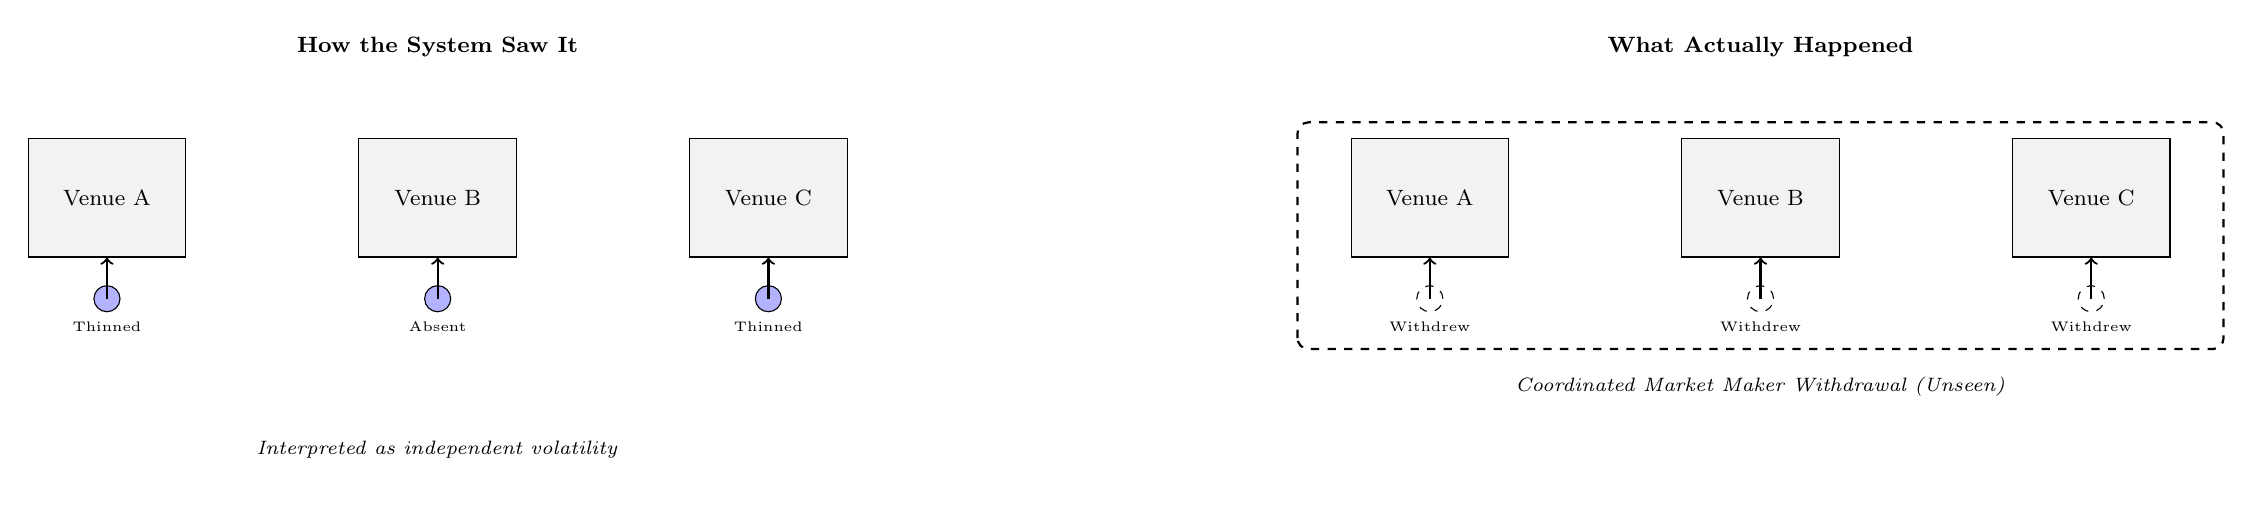
\begin{tikzpicture}[
      font=\footnotesize,
      venue/.style={rectangle, draw, fill=gray!10, minimum width=2cm, minimum height=1.5cm, align=center},
      mmaker/.style={circle, draw=black, fill=blue!30, minimum size=4pt},
      ghost/.style={circle, draw=black, dashed, minimum size=4pt},
      arrow/.style={->, thick},
      x=2.8cm, y=1.6cm
    ]

    % Labels
    \node at (1.5, 3.2) {\textbf{How the System Saw It}};
    \node at (7.5, 3.2) {\textbf{What Actually Happened}};

    % System View Venues
    \node[venue] (v1) at (0,2) {Venue A};
    \node[venue] (v2) at (1.5,2) {Venue B};
    \node[venue] (v3) at (3,2) {Venue C};

    % Actual View Venues
    \node[venue] (v4) at (6,2) {Venue A};
    \node[venue] (v5) at (7.5,2) {Venue B};
    \node[venue] (v6) at (9,2) {Venue C};

    % System View market makers
    \node[mmaker, label=below:\tiny Thinned] at (0,1.2) {};
    \node[mmaker, label=below:\tiny Absent] at (1.5,1.2) {};
    \node[mmaker, label=below:\tiny Thinned] at (3,1.2) {};

    % Actual View: All withdrew
    \node[ghost, label=below:\tiny Withdrew] at (6,1.2) {};
    \node[ghost, label=below:\tiny Withdrew] at (7.5,1.2) {};
    \node[ghost, label=below:\tiny Withdrew] at (9,1.2) {};

    % System View arrows
    \draw[arrow] (0,1.2) -- (v1.south);
    \draw[arrow] (1.5,1.2) -- (v2.south);
    \draw[arrow] (3,1.2) -- (v3.south);

    % Actual View arrows
    \draw[arrow] (6,1.2) -- (v4.south);
    \draw[arrow] (7.5,1.2) -- (v5.south);
    \draw[arrow] (9,1.2) -- (v6.south);

    % Dotted enclosure for actual coordinated retreat
    \draw[dashed, thick, rounded corners] (5.4,0.8) rectangle (9.6,2.6);
    \node at (7.5, 0.5) {\textit{\scriptsize Coordinated Market Maker Withdrawal (Unseen)}};

    % Explanation notes
    \node at (1.5, 0) {\textit{\scriptsize Interpreted as independent volatility}};
    \node at (7.5, -0.2) {};

    \end{tikzpicture}%
  }
  \caption{System vs. Reality: The aggregator saw isolated venue stress. In truth, liquidity withdrew systemically.}
\end{figure}


  


\textbf{The flaw wasn’t technical failure. It was logic working as designed, but under the wrong conditions.}

\textbf{The aggregator routed into a void, not because it was broken — but because it believed the market was still there.}

That’s the most dangerous kind of system failure: the one that still works.

The pipes were connected. The APIs responded. The venues echoed back confirmations.  
But what the system couldn't see — or refused to infer — was that the liquidity had quietly vanished.

It was like shouting into a canyon that used to be a city, and hearing your own voice bounce back.  
The echo sounded familiar. But no one was there anymore.

\medskip

\textbf{Analogy 1: A Self-Checkout Lane With No Inventory}

Imagine walking into a grocery store during a supply chain crisis.  
The lights are on. The checkout scanner works. The receipt prints.  
But the shelves are empty.

The system isn’t broken — it’s just useless.  
It tells you “transaction complete,” even though the bag is empty.

That’s what the aggregator did: it kept sending tranches into “functioning” venues, mistaking a live connection for a live market.

\medskip

\textbf{Analogy 2: Calling a Number That Goes to Voicemail}

You call your friend. It rings. You assume they’re busy — so you keep calling.  
But they changed their number days ago.  
You’re not getting through — you're hearing a ghost.

\medskip

\textbf{Analogy 3: Following GPS Into an Abandoned Town}

Your GPS guides you into what it believes is a busy town center.  
You follow — and find empty roads and shuttered stores.

The roads are real. The signs are intact. But the town has died.

\medskip

\textbf{That’s what happened here.}

The aggregator didn’t crash.  
It performed exactly as designed — assuming the market was real.

But the market was a mirage.  
And in trusting the echo, it slipped — quietly, repeatedly — until the losses were booked.

  

\begin{figure}[H]
  \centering
  \begin{tikzpicture}[
    venue/.style={rectangle, draw, minimum width=2.5cm, minimum height=1cm, fill=gray!10},
    aggregator/.style={ellipse, draw, minimum width=3.5cm, minimum height=1.2cm, fill=blue!10},
    arrow/.style={->, thick},
    dashedarrow/.style={->, thick, dashed},
    annotation/.style={font=\small\itshape}
  ]

  % Aggregator node
  \node[aggregator] (agg) at (0,0) {Synthetic Aggregator};

  % Venue nodes
  \node[venue] (v1) at (-5,-3) {Venue A};
  \node[venue] (v2) at (-2,-3) {Venue B};
  \node[venue] (v3) at (1,-3) {Venue C};
  \node[venue] (v4) at (4,-3) {Venue D};

  % Arrows from aggregator to venues
  \draw[arrow] (agg.south) -- (v1.north) node[midway, left, xshift=-0.3cm] {\tiny tranche 1};
  \draw[arrow] (agg.south) -- (v2.north) node[midway, left] {\tiny tranche 2};
  \draw[arrow] (agg.south) -- (v3.north) node[midway, right] {\tiny tranche 3};
  \draw[arrow] (agg.south) -- (v4.north) node[midway, right, xshift=0.3cm] {\tiny tranche 4};

  % Failing venue indicators
  \node[annotation] at (-5,-4) {no fill};
  \node[annotation] at (-2,-4) {partial fill};
  \node[annotation] at (1,-4) {slow fill};
  \node[annotation] at (4,-4) {timeout};

  % Dashed arrows to indicate aggregator misinterpretation
  \draw[dashedarrow, red] (v1.north east) .. controls (-4,0) .. (agg.south west);
  \draw[dashedarrow, red] (v4.north west) .. controls (3,0) .. (agg.south east);

  % Label at bottom
  \node[annotation, align=center] at (0, -5) 
  {Aggregator continued routing in smaller tranches \\ assuming liquidity would rebound};

  \end{tikzpicture}
  \caption{Synthetic Aggregator disperses tranches to multiple venues — unaware that systemic liquidity is collapsing.}
\end{figure}

\textbf{Dark Pool and OTC Failover \textemdash\ Silent Continuity Breakdown}

  \textbf{Dark Pool and OTC Failover} is the final layer in a multi-tiered trade execution architecture. It is designed 
  to handle 
  \textit{large block orders} when traditional lit venues (like NYSE or ARCA) and smart aggregation routes are 
  either stressed or unavailable.
  
  \medskip
  
  \textbf{The Intended Design}

  The architecture was built as a three-layered system — like a triage protocol or a multi-lane highway — with each 
  layer designed to handle escalating levels of market stress:
  
  \begin{itemize}
  
    \item \textbf{Primary Venues: Fast, liquid markets for baseline execution.}
  
    These include major exchanges like NYSE, NASDAQ, and ARCA — fast, deep, and efficient. The system was designed 
    to route most trades here under normal conditions.
  
    \textit{Analogy:} Think of these as the express lanes on a freeway. Well-lit, always flowing. You expect them to 
    carry most of the traffic smoothly. That’s where you send your orders first.
  
    \medskip
  
    \item \textbf{Synthetic Aggregator: Tranche-based smart routing across smaller venues.}
  
    This layer activates when primary venues thin out. It breaks up large trades into smaller slices — tranches — 
    and spreads them across smaller venues (regional exchanges, ECNs, dark pools). These pieces are then reassembled 
    to approximate optimal execution.
  
    \textit{Analogy:} It’s like ordering a meal that’s split between multiple nearby restaurants using a delivery app. 
    Each kitchen handles a part of the order, and you get the full meal stitched together. It’s adaptive, efficient — 
    but only if all kitchens are still working.
  
    \medskip
  
    \item \textbf{Dark/OTC Layer: Reserved for emergency or high-impact blocks.}
  
    This is the backup circuit — used only when other layers show signs of structural stress. It handles large trades 
    discreetly, either through dark pools or negotiated OTC desks.
  
    \textit{Analogy:} It’s like buying a thousand cases of wine. You don’t go to the grocery store. You contact a private 
    distributor off the showroom floor. Quiet, efficient, and high-capacity — but not designed for routine traffic.
  
  \end{itemize}
  
  \bigskip
  
  \textbf{Together, the system formed a layered failover stack:}
  
  \begin{itemize}
    \item Use the main exits first (primary venues).
    \item If blocked, break into smaller groups and use side stairwells (synthetic aggregator).
    \item If the building’s on fire, trigger the emergency slide (dark/OTC layer).
  \end{itemize}
  
  \medskip
  
  \textbf{The failure wasn’t architectural.}  
  All the layers were there. The flaw was interpretive.
  
  The system couldn’t recognize that the main exits weren’t just congested — they were missing. It read structural 
  breakdown as temporary volatility. And by the time it reached for the backup chute, the fire had already spread.

  \begin{figure}[H]
    \centering
    \resizebox{0.65\textwidth}{!}{%
      \begin{tikzpicture}[
        font=\small,
        layerbox/.style={draw, thick, rounded corners, minimum width=6cm, minimum height=1.2cm, align=center, fill=gray!10},
        arrow/.style={->, thick},
        metaphor/.style={font=\scriptsize\itshape},
        yscale=1.5
      ]
  
      % Layers
      \node[layerbox] (primary) at (0, 4) {
        \textbf{Primary Venues}\\
        Fast, liquid markets for baseline execution
      };
      \node[metaphor, below=0.1cm of primary] {“Freeway express lanes”};
  
      \node[layerbox] (synthetic) at (0, 2) {
        \textbf{Synthetic Aggregator}\\
        Tranche-based routing across fragmented venues
      };
      \node[metaphor, below=0.1cm of synthetic] {“Split delivery from nearby kitchens”};
  
      \node[layerbox] (otc) at (0, 0) {
        \textbf{Dark / OTC Layer}\\
        Reserved for emergency or high-impact blocks
      };
      \node[metaphor, below=0.1cm of otc] {“Private wine distributor off the floor”};
  
      % Arrows
      \draw[arrow] (primary.south) -- (synthetic.north);
      \draw[arrow] (synthetic.south) -- (otc.north);
  
      % Optional: Fallback logic label
      \node at (3.2, 2) {\rotatebox{90}{\textbf{Failover Path}}};
  
      \end{tikzpicture}%
    }
    \caption{Layered Execution Stack: The system was designed to cascade from fast primary venues, to synthetic 
    aggregation, to dark/OTC channels as fallback.}
  \end{figure}
  
  


  
  
  
  
  \medskip
  
  \textbf{What failed:}
  \begin{enumerate}
    \item \textbf{Primary venue didn't crash \textemdash\ it thinned silently.} Top bids were pulled, depth 
    vanished, but the exchange stayed online. Latency monitors remained within thresholds, so the system saw 
    no problem.
  
    \item \textbf{Synthetic aggregator misclassified the event.} It interpreted the pullback as transient 
    volatility, not structural withdrawal of liquidity. It continued routing partial tranches, assumed spreads 
    would re-converge, and reported degraded but valid execution.
  
    \item \textbf{Dark/OTC logic never activated.} Because:
    \begin{itemize}
      \item Synthetic routing was still returning partial fills ("success")
      \item Slippage increased gradually, but was interpreted as price movement
      \item No upstream system raised a critical alert
    \end{itemize}
  
    Thus, \textit{fallback thresholds were never crossed}.
  \end{enumerate}
  
  \medskip
  
  \textbf{The consequence:} A silent, cascading misalignment:
  \begin{itemize}
    \item The first layer \textbf{lost depth}, but stayed online.
    \item The second \textbf{misread stress} as benign volatility.
    \item The third \textbf{remained dormant} \textemdash\ because the upstream logic didn’t scream.
  \end{itemize}
  
  \medskip
  
  \textbf{This was not a crash.} It was a \textit{quiet continuity failure}, where automated systems masked degradation 
  through technical functionality.
  
  \medskip
  
  \textbf{Key Risk:} \emph{Fallback logic that works too well.}
  If every layer silently adapts, no one intervenes \textemdash\ until the damage is already booked.

  



\begin{figure}[H]
  \centering
  \begin{tikzpicture}[
    font=\small,
    thick,
    node distance=2.2cm and 1.5cm,
    event/.style={draw, rectangle, rounded corners, fill=gray!10, text width=4.2cm, align=left, minimum height=1.2cm},
    arrow/.style={-{Stealth}, thick},
    dashedarrow/.style={-{Stealth}, thick, dashed}
  ]

  % Timeline nodes
  \node[event] (primary) 
    {\textbf{Primary Venue Execution}\\
    Bids pulled, depth vanished — but latency stayed in range, so no alert.};

  \node[event, below=of primary] (synthetic) 
    {\textbf{Synthetic Aggregator Layer}\\
    Interpreted thinning as volatility. Continued routing in tranches. Misread structural exit.};

  \node[event, below=of synthetic] (dark) 
    {\textbf{Dark Pool / OTC Failover}\\
    Never triggered — upstream reported “success.” Slippage mistaken for normal price action.};

  % Arrows
  \draw[arrow] (primary) -- (synthetic);
  \draw[arrow] (synthetic) -- (dark);

  % Misinterpretation annotations
  \node[align=left, text width=5.5cm, right=2cm of primary] (a1) {
    \textit{Behavioral Signal:} Venue “online” \\
    \textit{Technical Reading:} No spike in latency \\
    \textit{Result:} Assumed healthy
  };
  \draw[dashedarrow] (primary.east) -- (a1.west);

  \node[align=left, text width=5.5cm, right=2cm of synthetic] (a2) {
    \textit{Behavioral Signal:} Tranches filling erratically \\
    \textit{Technical Reading:} Normal market thinning \\
    \textit{Result:} Kept routing
  };
  \draw[dashedarrow] (synthetic.east) -- (a2.west);

  \node[align=left, text width=5.5cm, right=2cm of dark] (a3) {
    \textit{Behavioral Signal:} Losses rising slowly \\
    \textit{Technical Reading:} No threshold breach \\
    \textit{Result:} Never escalated
  };
  \draw[dashedarrow] (dark.east) -- (a3.west);

  \end{tikzpicture}
  \caption{Timeline of Silent Degradation Across Fallback Layers}
\end{figure}

  







